\documentclass{article}

\usepackage[hscale=0.8,vscale=0.8]{geometry}
\usepackage{graphicx}
\usepackage{amsfonts, amsmath, amsthm, amssymb} % For math fonts, symbols and environments



\pagenumbering{gobble}

\author{Finnian Lattimore}
\title{Causal Inference in one page}

\begin{document}
\def\ci{\perp\!\!\!\perp}

\subsection*{Causal Inference without the do-opperator}



One way we can encode our assumptions about the state of the world now and how a given intervention modifies that state is with graphical models. Specifically, assume that the data we have is generated from a directed acyclic graph (DAG) and that we know the structure of the graph (although we may not be able to observe all the variables). An arrow $A \rightarrow B$ means $A$ causes $B$. 

If we intervene in the system and force a particular variable, $X$ to some value, $x$, the result is a new graph that is identical to the original one except that the conditional probability distribution associated with $X$ is replaced by $X=x$ and any links coming into $X$ are removed (since under the assumption that some external intervention is forcing $X=x$ it will no longer depend on its original causes). The classic example for the question of the causal effect of smoking on lung cancer is shown in figure XXX. 

We want to estimate the probability of cancer given smoking after the intervention (ie in the graph $G_X$) using observational data (data generated by the original model $G$). The problem of causal inference in general is to determine if it is possible to estimate the desired conditional probabilities in the graph representing the system after a given intervention from conditional probabilities in the original graph. 

This can be determined by repeated applications of Pearl's 3 rules, which we will restate (without the do notation). For simplicity we will only consider the effect of intervention on a single variable, $X$, on a single target $Y$. 

\subsubsection*{Rule 1}
 D-separation still applies in the graph $G_X$:
 
 \begin{equation}
 Y \text{ d-sep } W \text{ given } Z \text{ in } G_X \implies P_{G_X}(Y|Z,W) = P_{G_X}(Y|Z)
 \end{equation}

\subsubsection*{Rule 2}
If, after conditioning on $Z$, $G$ and $G_X$ have exactly the same active trails between $X$ and $Y$ then $P(Y|X,Z)$ will be the same in both graphs $P_G(Y|X,Z) = P_{G_X}(Y|X,Z)$.
 
  
Equivalently, we can state this in terms of D-separation by adding an additional variable $\hat{X}$ as a parent of $X$ in the original graph. If $\hat{X}$ d-sep $Y$ given $X$ and $Z$ in $G$ then there are no active trails from $X$ to $Y$ that begin with an arrow into $X$. This means no active trails will be removed in the process of creating graph $G_X$. You can think of the variable $\hat{X}$ as a switch that determines if $X$ takes its value as determined by its other parents or from some external source. 

\begin{equation}
Y\text{ d-sep }\hat{X}\text{ given }X,Z \implies P_G(Y|X,Z) = P_{G_X}(Y|X,Z)
\end{equation}
 
\subsubsection*{Rule 3}
If, after conditioning on $Z$, the only active trails from $X$ to $Y$ in the original graph $G$ begin with an arrow pointing into $X$ then $Y$ will be independent of $X$ given $Z$ after the intervention (since we will have deleted all the arrows going into $X$). 

Stated in terms of D-separation:
\begin{equation}
Y \text{ d-sep } \hat{X} \text{ given } Z \implies P_{G_X}(Y|X,Z) = P_{G_X}(Y|Z)
\end{equation}



\subsubsection*{These rules are complete}
We can estimate the conditional distribution of interest in $G_X$ if and only if we can re-write it in terms of observable conditional independences in $G$ via repeated application of these rules.

You might have been hoping for a single, simple graphical criterion for identification - but sadly, to my knowledge, there isn't one. There are some that are sufficient and some that are necessary - but none that are both.


\subsubsection*{The causal effect of smoking}







 





\subsection*{Causal Inference}
Causal inference covers problems where we want to predict the outcome of an intervention given some known causal structure
\begin{itemize}
\item Assume that the true causal structure is a directed graphical model where $X \rightarrow Y$ means $X$ causes $Y$. We know the structure of the network but may not be able to observe the values of all the variables.
\item Intervening to set $X = x$, denoted $do(X=x)$ in a causal network, has the effect of removing all links coming into the variable $X$ (since its value is no longer determined by its parents) and setting its value to $x$.
\item We can use d-separation to derive the 3 rules of the do-calculus that allow us write queries about interventions in terms of the pre-interventional distribution. 
\item These rules are complete.  If an expression containing do's can be converted into one that does not by repeated application of the rules then you can determine the post-interventional distribution from observational data. If you can't, its not possible without additional assumptions.
\end{itemize}
The rules (simplified to cover only the case where we intervene on a single variable) can all be illustrated by the graph in figure \ref{fig:dorules}. Assume our query is $P(Y|do(X))$. $G^{\dagger}$ is the original graph, $G$, augmented to include a variable $\hat{X}$  that acts as a switch determining if $X$ takes its value as determined by its parents or from an external intervention. $G_{\overline{X}}$ is $G$ after the intervention. 

\begin{figure}[h]
\caption{The do calculus}
\label{fig:dorules}
\centering
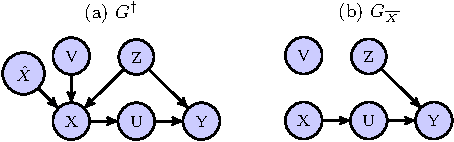
\includegraphics[scale=0.9]{do_rules_figure-crop}
\end{figure}

\begin{enumerate}
\item D-separation still applies after an intervention. $Y \ci V|X$ in $G_{\overline{X}}$ $\implies P(Y|do(X),V) = P(Y|do(X))$
\item If the outcome variable is independent of the way in which the intervened on variable takes its value, intervention = observation. $Y \ci \hat{X}|X,Z$ in $G^{\dagger} \implies P(Y|do(X),Z) = P(Y|X,Z)$
\item If there is no direct path from the intervened on variable to the outcome variable, the intervention does not effect the distribution of the outcome variable. $Y \ci \hat{X}|U$ in  $G^{\dagger} \implies P(Y|do(X),U) = P(Y|U)$
\end{enumerate}
In figure \ref{fig:dorules} we can identify the causal effect of $X$ on $Y$ provided we can observe either $Z$ or $U$.

Key general references: \cite{Pearl2000,Koller2009}

\subsection*{Causal Structure Learning - learn causal structure from observational data}
\subsubsection*{Conditional independence approach} 

\begin{itemize}
\item Assume that the data was generated by an unknown causal directed graphical model
\item Assume that all dependencies in the graph are reflected by conditional dependencies in the distribution of the data (ie no dependencies exactly cancel one-another out) $\leftarrow$ faithfullness assumption
\item Finding the true causal structure is equivalent to finding the set of graphs that are perfect maps for the data distribution. In general, result is not unique but some links may have the same direction in all graphs in the set.
\item Approach can be extended to allow for latent variables
\item Key general reference: \cite{Sprites}
\end{itemize}
\subsubsection*{Functional form approach}
Conditional independence based methods cannot distinguish between graphs with the same dependency structure, for example,  $X \rightarrow Y$ vs $Y \rightarrow X$. We can infer causality in such cases if we make braod assumptions about the relationship between the function mapping cause to effect and any noise. Suppose $X \rightarrow Y$:
\begin{itemize}
\item If we assume noise is additive in the causal direction, $Y = f(X)+\epsilon$ cannot generally be inverted to give an additive model in the other direction (linear $f$ and gaussian $\epsilon$ are an unfortunate exception)\cite{Hoyer2009}.
\item If $f$ is deterministic and invertible, for most input distributions $p_X(x)$ the distribution of $p_Y(y)$ will be higher where $f'$ is small and a large region of $X$ maps to similar values of $Y$. We expect that $f$ and $p_X$ are independent but $f'$ and $p_Y$ are correlated \cite{Daniusis2010}.
\item In general, $P(X)$ and $P(Y|X)$ should be independent but $P(Y)$ and $P(X|Y)$ will not be \cite{Scholkopf2012}
\end{itemize}

\bibliographystyle{plain} % Plain referencing style
\bibliography{library} % Use the example bibliography file sample.bib
\end{document}